\chapter{Our approach}
\label{chap:math}

\section{Design choices}
One design choice was to let the end user decide to build ART with or without Embree support. Since ART is build with CMake, a Boolean CMake variable \texttt{ENABLE\_EMBREE\_SUPPORT} was introduced, so that if one wishes to build ART with Embree support, he or she has to invoke 

\begin{lstlisting}[language=bash]
$ cmake -DENABLE_EMBREE_SUPPORT=1 
\end{lstlisting}

The rest of the building procedure is identical to the one described in the user documentation of ART \cite{arthandbook}.

The second crucial design choice was to introduce a single class called "ArnEmbree", which should provide the necessary functionality concerning Embree, e.g. the creation and deletion of an Embree scene, the adding of different scene geometry and performing the intersection calculations with Embree. This file should act as a singleton object. To quote from ART's user manual \cite[Chapter 4.1.2]{arthandbook} "Apart from this struct, [the \texttt{art\_gv} global variable] there are no genuine global variables in ART, only global constants". The singleton object obviously contradicts this statement. However, an inclusion of an ArnEmbree singleton to the \texttt{art\_gv} variable should is possible and probably not too difficult. During the development, Embree functionality is kept separate from \texttt{art\_gv}.

Finally, while being in an "experimental state", the inclusion of Embree in ART was designed in a way that "native" rendering with ART should still be supported. Therefore, even if ART was build with Embree support, one has to add the flag \texttt{-e} or \texttt{--embree}. For example, rendering the scene file \texttt{foo.arm} with Embree can be done by the command 

\begin{lstlisting}[language=bash]
$ artist foo.arm -e 
\end{lstlisting}

as opposed to the command

\begin{lstlisting}[language=bash]
$ artist foo.arm
\end{lstlisting}


\section{Types of Shapes in ART}

ART supports a variety of different geometrical shapes. An overview of these shapes can be found in the "ARM File Reference Manual" \cite{artreferencemanual}.The shapes are divided by ART into two categories: \emph{Shapes} and \emph{Simple Indexed Shapes} (to avoid confusion, the Shape type will be referred to as \emph{Regular Shape} throughout the thesis). Simple Indexed Shapes are quadrangles and triangles. To each simple indexed shape, an array of 3D points and and an array of face indices is associated with it, which is sufficient to describe them in 3D space. 
Regular Shapes on the other hand do not require an index array but further information. 

\begin{figure}[!tbp]
	\centering
	\subfloat[Triangle shape.]{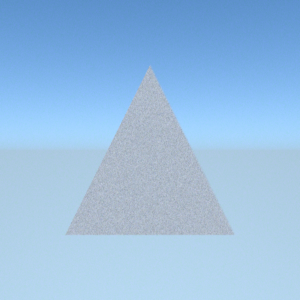
\includegraphics[width=.3\textwidth]{img/3 approach/triangle.png}\label{fig:art_triangle}}
	\hfill
	\subfloat[Torus shape alligned on Y-axis.]{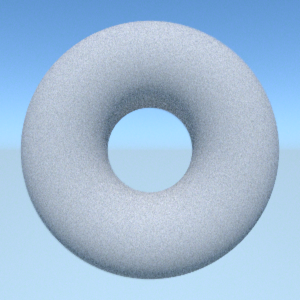
\includegraphics[width=.3\textwidth]{img/3 approach/torus.png}\label{fig:art_torus}}
	\caption{My flowers.}
\end{figure}


